% vim: set tw=78 sts=2 sw=2 ts=8 aw et ai:

Initially, the architecture of our open source machlib had the following
architecture:

\begin{figure}[H]
  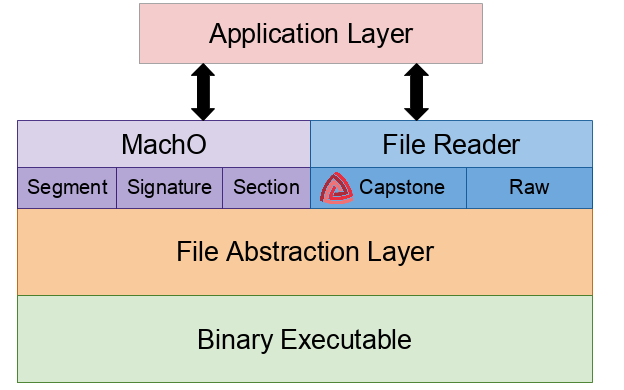
\includegraphics[scale=0.4]{MachoArch1.png}
  \centering
\end{figure}

We can notice that the API is defined by two classes, namely MachO and
FileReader, which together expose functionality to the userspace. The
foundation that these two classes rest on remaines unchanged for now.

Nevertheless, an important change has occured in the archiecture of our
library: the entry point has changed from the MachO class, to the
UniversalBinary class, which is a more general abstraction of a MachO
executable:

\begin{figure}[H]
  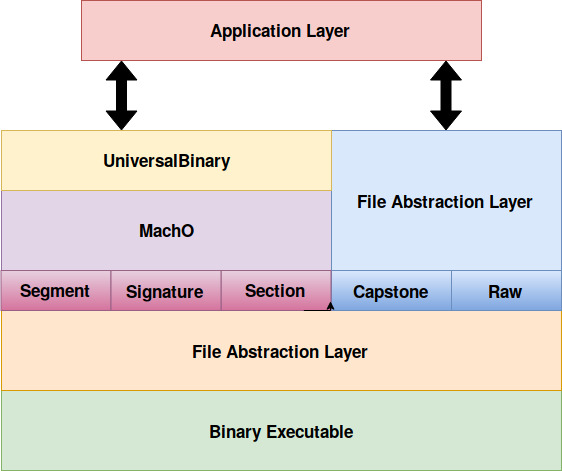
\includegraphics[scale=0.4]{MachoArch2.jpg}
  \centering
\end{figure}

Basically, the UniversalBinary class wraps both the concept of a fat binary,
as well as that of a simple binary (containing code for only one
architecture).

The final API is yet to be defined, even though the current state of the
project has a working fat header and far architecture header parser.
